\chapter{Method}
\label{ch:methods}

\noindent In this chapter, the contributions proposed and applied during this thesis are discussed.
The proposed architecture defined in Chapter \ref{ch:setup} is shown.
Afterwards, the experiment configuration is described.% to show how the proposed methodology addresses the research goals.
Finally, the localisation and mapping models are presented, along with their respective evaluation techniques.

\section{Proposed Architecture} 
\label{ch:prop-architecture}
\noindent The proposed architecture for the final system is shown in Figure \ref{fig:arch-structure}. 
The localisation module is defined using a sensor fusion filter.
%This approach exploits available measurements, hence limiting the drawbacks of individual sensors and highlighting their contributions.
The proposed approach is an \gls{EKF}, chosen due to its robust and adaptable nature.
The \gls{EKF} enables for fast and reliable fusion of heterogeneous sensors in a way that allows the \gls{ALM} to have a real-time and accurate estimate of its pose.
The mapping module is defined using the results of the localisation as a baseline, and exploiting the collision detection measurements of the \gls{ALM}.
Through the use of these components, a virtual boundary is created and the presence of objects within it will be provided by the events fired by the collision sensors.
%Finally, the methodology adopted to evaluate the performances of these modules is defined. \{where is this defined? Maybe cut this sentence}
\begin{figure}[H]
	\begin{center}
	\centering
		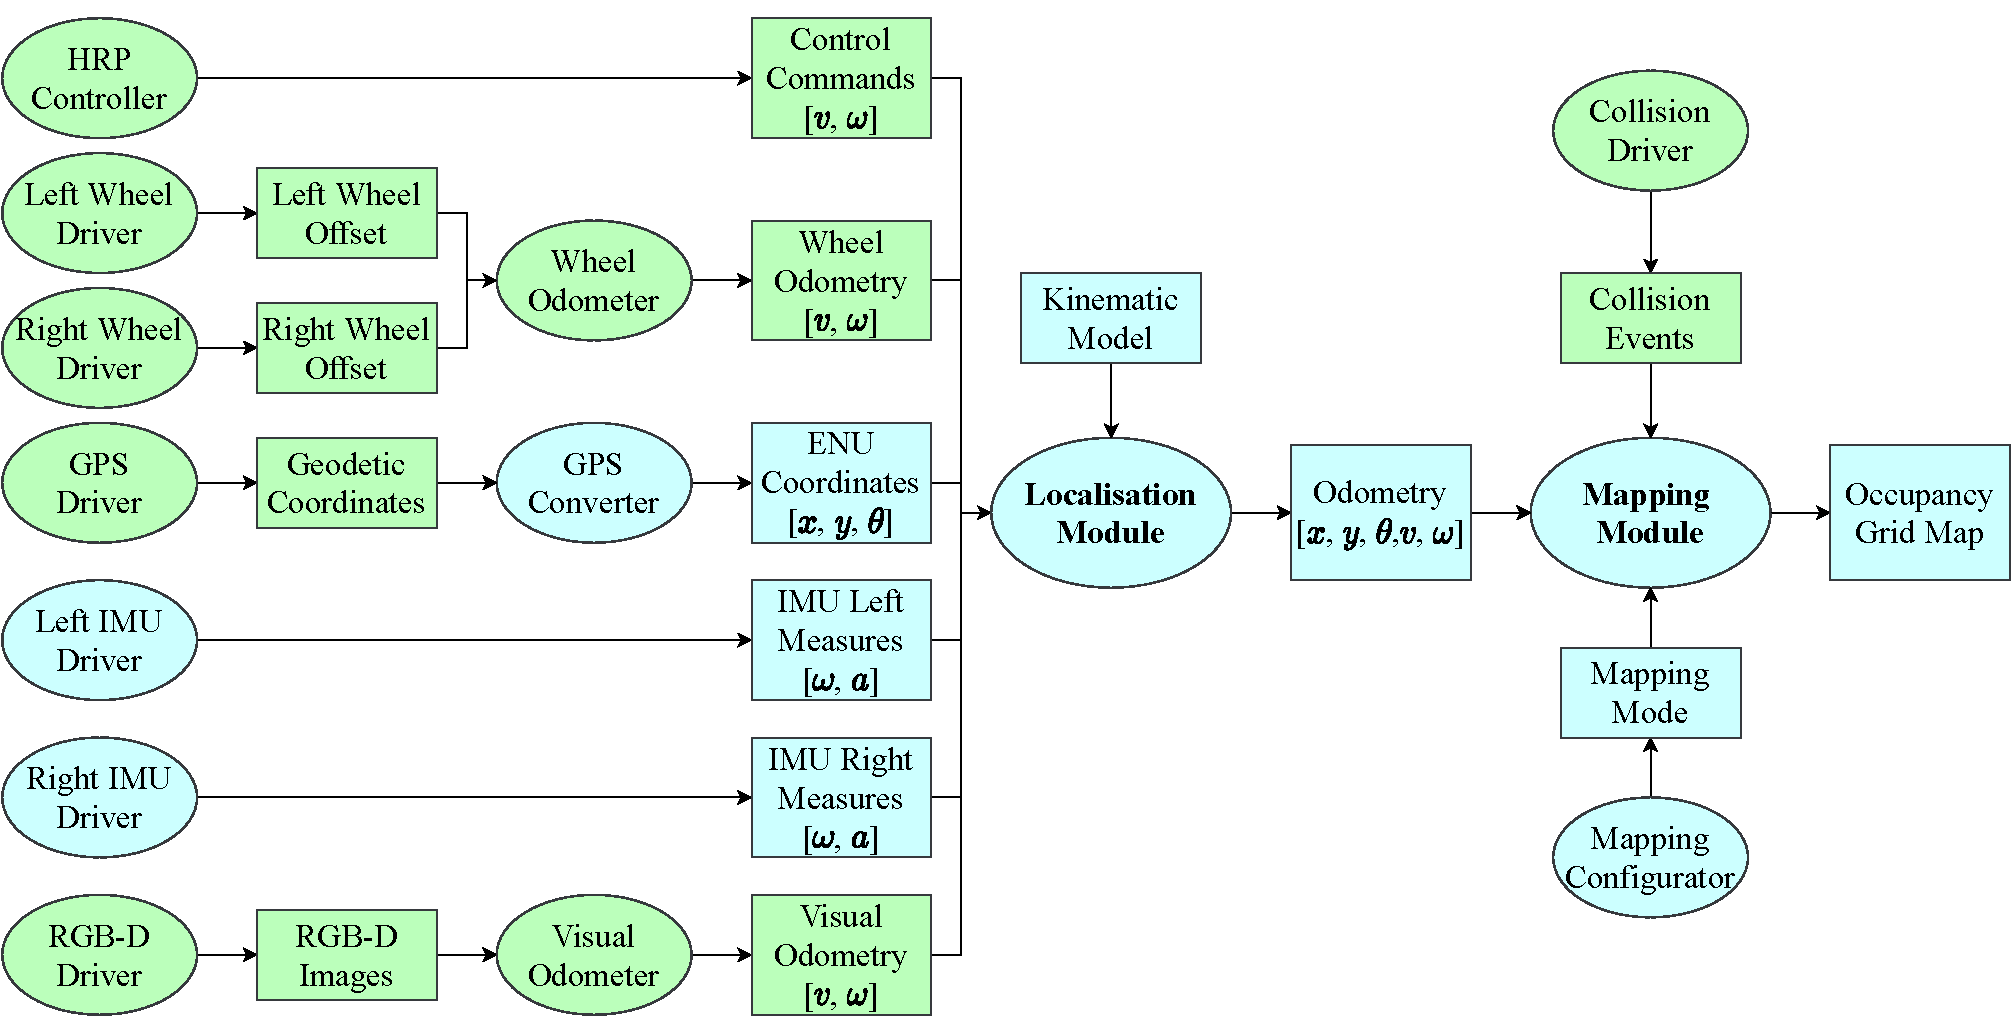
\includegraphics[width=1\textwidth]{Images/3-0-SetUp/SWSetUp.pdf}
		\caption{Software nodes(ellipses) and data structures(rectagles) including\\
		both available(green) and newly developed(blue) components.\\
		In bold the main contributions.\centering }
		\label{fig:arch-structure}
	\end{center}
\end{figure}
\section{Experiments}
\noindent The proposed architecture will be evaluated using multiple experiments, in which the \gls{ALM} is teleoperated by an external computer interacting with the \gls{HRP} Controller.
It sets the control commands as the linear and angular velocities, as defined during the kinematic analysis in Section \ref{ssec:kin_a}.

Some initial training tests are run to check the system's integrity and the correct interaction of the modules.
The data gathered in these multiple outdoor runs is then used to test and analyse the performance of the system.
Some tests have been made to define the calibration of the sensors against a ground truth identified using measure tape.
Other runs checked an accurate system's behaviour while steering.
Final tests ensured that the collision events are estimated with a certain degree of precision.

After this first phase, the proposed system's architecture is analysed with a testing run on gravel and a validation run on grass.
Each experiment will consist of both the localisation and mapping modules.
%Regarding the localisation topic, the experiments will be evaluated using different sensors' configurations.
The evaluation of the different sensors' configurations are performed in a successive phase of the experiment.
During the outdoor runs, the input measurements from the sensors are registered.
In a second moment, the results are replayed to compute the system's performance and to analyse which of their possible configurations provided the best results.
%The analysis will be conducted separately for the modules and their related evaluation metrics used for each respective component are described in the following sections. 

The results are considered valid if they show that the same methodology adopted provides similar results in different settings.
The methodology adopted during the training of the filter is then tested in the validation experiment to ensure that the performances are indifferent to the environment.
%The method is valid if the simulation filtering provide values close to the ground truth with the same configuration.%, showing that if the assumptions are validated then the system behaves as best estimator.


\subsection{Gravel Testing Experiment}
\noindent
The testing experiment has been run on a parking lot with gravel floor.
It has been used to test the first complete configuration of the \gls{ALM}.
In this case, only the boundary setting on the mapping module has been implemented.

\subsection{Grass Validation Experiment}
\noindent
The final validation has been made on a park with tall grass to test a more realistic scenario.
The sensor fusion localisation and the occupancy grid mapping have been run together using the findings of the gravel test.
Furthermore, the complete mapping module has been adopted. 

\subsection{Ground Truth Generation}
\label{sec:gt}
\noindent The ground truth is constructed manually by checking the actual path travelled by the robot with the usage of a measure tape properly set during the experiments.
The values obtained are then used to generate a dynamic virtual run which follows the real run as it was carried out in reality, which is finally adopted to check the system's performance.

\section{Localisation}
\label{sec:loc-method}
\noindent The Localisation Module is based on a \gls{EKF} which unifies and fuses the information derived by the kinematic model, the control commands, and the sensors' measurements.
It has been selected and adopted for its time performances and reliability.
As analysed in~\cite{801027}, the performance of a \glspl{KF} driven by the kinematic model are similar to the one obtained by a filter driven by the \gls{WO} measurements.
However, as in this project the control commands are also available, the Prediction phase is defined by the kinematic model while the \gls{WO} measurements are used by the \gls{EKF} for the Correction phase.

The filter works with a discretised time system which is executed with a frequency of \SI{250}{Hz}, which is the highest sampling frequency among the sensors, obtained by the \glspl{IMU}.
%It improves the \gls{KF} allowing for the management of non-linear systems and the possibility to account for dynamic sensors' noise.
At first, the Prediction step is computed, using the sampling period, while the system gathers new sensors' measurements, which are used to dynamically create the components for the Correction step. 
After a delay has been waited to reach the desired frequency rate, the Correction step merges the measurements into the filtered state and covariance before reiterating this procedure. 
%Check
The execution of the steps is not immediate, as it needs some time consuming computations, so the sampling rate of the \gls{EKF} is variable and the related time step is defined dynamically by the varying $\boldsymbol \Delta_t$.
The algorithm will use this varying sampling period at each prediction step to accurately transition the filtered estimate into the discretised predicted estimate defined by this value. 

\subsection{Calibration Step}
\noindent
Before starting to fuse the data for the sensors, an initial phase of calibration for some sensors is necessary.
In this preliminary step, the measurements obtained from some sensors are used to elaborate a value that will be later adopted in their covariance measurement matrices $R_*$, used to weight the relevance of their measurements in the correction phase. %provide on their own the variance of all their estimates.
This step is needed to ensure that the \gls{EKF} will behave properly in different ground conditions.

This operation is needed by the wheel encoders and by the \gls{GPS} receiver as their variances are not disclosed.
The calibration of the GPS receiver is derived after five minutes of stationary state.
During this period, the provided \gls{HDOP} error rate, which is obtained internally using the pseudoranges measurements, is scaled to match the variances estimated from its initial fix in the local frame. 
This scaling value is then used throughout the entire test to adapt the varying \gls{DOP} estimate into a varying \gls{GPS} measurement covariance matrix.
The position estimates derived from this still pose are also averaged to provide the initial reference fix adopted by the \gls{GPS} measurement model to compute its local position.
The wheel encoders compute their variances using the measurements obtained by moving the \gls{ALM} in a sample run of \SI{5}{meters} before the test. 
The obtained calibration variances are adopted by the wheel encoder measurement covariance matrix.
The initial calibration run is also exploited by the \gls{GPS} measurement model used to compute the variance of the orientation estimates obtained as defined in \ref{sec:gps-rec-mod}.


\subsection{Prediction Model}

\noindent The prediction phase is driven by the kinematic model and the eventual control commands, as defined in Figure \ref{fig:TikzKine}.
It has been adopted given its better performance with respect to the odometer driven model~\cite{801027}.

After the calibration phase, the \gls{ALM} is in a stationary state.
The system will then start with all its state variables $\mathbf{X}_0^-$ set to $0$.
The initial Covariance matrix $P_0$ is set as the identity matrix multiplied by $1^{-3}$.

The state variables needed to provide the most accurate positioning in a \gls{2D} environment are defined in \eqref{eq:state-transf}:
\begin{equation}
	\label{eq:state-transf}
	\mathbf{X}_t =
	\begin{bmatrix}
		\mathbf{x}_t & \mathbf{y}_t & \boldsymbol \theta_t & \mathbf{v}_t & \boldsymbol \omega_t
	\end{bmatrix} ^T
\end{equation}
From the definition of the Kinematic Model in Figure \ref{fig:TikzKine}, the first three positional elements, i.e., $\mathbf{x}_t$, $\mathbf{y}_t$, and $\boldsymbol \theta_t$, are related to the global frame. 
Instead the following inertial elements, i.e., $\mathbf{v}_t$ and $\boldsymbol \omega_t$ are defined from the robot frame.
As assumption, the system will start with a known initial state $\mathbf{X}_0$ of mean $0$ for each element, and it will follow a Constant Velocity model.

%\subsubsection{Transition}
The transition matrix related to the states defined in Equation \eqref{eq:state-transf} and to the kinematic model of Figure \ref{fig:TikzKine} is presented below:
\begin{equation}
	\label{eq:trans-mat}
	A_t
	=
	\begin{bmatrix}
		1 & 0 & 0 & \cos(\boldsymbol \theta_t) \cdot \Delta_t & 0 \\
		0 & 1 & 0 & \sin(\boldsymbol \theta_t) \cdot \Delta_t & 0 \\
		0 & 0 & 1 & 0 & \Delta_t  \\
		0 & 0 & 0 & 1 & 0 \\
		0 & 0 & 0 & 0 & 1 & 
	\end{bmatrix}
\end{equation}
where $\boldsymbol \theta_t$ is the orientation value of the current state and $\boldsymbol \Delta_t$ is the current sampling period used by the \gls{EKF} for the discretisation.
This model accounts for the transformation of the linear velocity and angular velocity to update the pose states defined in \eqref{eq:dof}.

%\subsubsection{Control}
As defined in Section \ref{ssec:kin_a}, the \gls{ALM} is controlled using the linear and angular velocities.
This configuration is used by the \gls{EKF} to complete the Prediction step using the following Control matrix $B$ and control state $\mathbf{u}_t$, as in:% Equations \eqref{eq:cmd}.
\begin{align}
	\label{eq:cmd}
	B &=
	\begin{bmatrix}
		0 & 0 \\
		0 & 0\\
		0 & 0\\
		s & 0\\
		0 & s
	\end{bmatrix}
	&
	\mathbf{u}_t &=
	\begin{bmatrix}
		\mathbf{v} - \mathbf{v}_t  \\
		\boldsymbol \omega - \boldsymbol \omega_t \\[0.3em]
	\end{bmatrix}
\end{align}
where $s$ is a smoothing factor adopted to make the transition from command received to actuation more realistic. %and  $\Delta_t$ is the varying time step of the \gls{EKF}, to dynamically define the matrix. 
%This smoothing matrix $B$ is adopted to avoid reaching the desired velocities sent to the robot , i.e., $\mathbf{v}$ and  $\boldsymbol \omega$. % obtained by a specific topic. 
%TODO Check
The control state $\mathbf{u}_t$ is defined as the difference between the control velocities desired, $\mathbf{v}$ and  $\boldsymbol \omega$, and the estimated velocities from the related state of $\mathbf{X}_t$.
This formulation enables the estimate to converge to the desired velocities in a time period defined by $F$, for which the chosen value for $s$ is set at each step as the value of the sampling period indicating that the filter will take indicatively a whole second to reach the desired velocities. %to ensure that including the control then the estimate will follow the desired value in the number of seconds defined by $F$.
\com{
	and $\mathbf{s}_{i}$ is used to make the transition from command received and actual actuation more smooth by limiting the innovation given by the respective control through a scaling value equal to the frequency of the system: $\mathbf{s}_i = \frac{1}{Hz}$, with $Hz$ as the frequency of the \gls{EKF}.
}

%\subsubsection{Uncertainty}
\com{
	The noise vector related to the state variables estimate is adaptively defined by $\boldsymbol \eta$ as in \eqref{eq:noise-p}.
	\begin{equation}
		\label{eq:noise-p}
		\boldsymbol \eta
		=
		\begin{bmatrix}
			\boldsymbol \eta_{\mathbf{x}}  &
			\boldsymbol \eta_{\mathbf{y}} &
			\boldsymbol \eta_{\boldsymbol \theta}  &
			\boldsymbol \eta_{\mathbf{v}} &
			\boldsymbol \eta_{\boldsymbol \omega} &
			\boldsymbol \eta_{\mathbf{a}}
		\end{bmatrix} ^T
	\end{equation}
	where $\eta_i \sim \mathcal{N}(\mu_i,\,\sigma_{ii}^{2})$ with $\mu_i = 0$, $\sigma_{ii}^2 = 0.1$, and $ i = \{ \mathbf{x} , \mathbf{y} , \boldsymbol \theta , \mathbf{v} , \boldsymbol \omega , \mathbf{a} \}$
	where $\sigma_{\mathbf{xx}}^2 = \sigma_{\mathbf{yy}}^2 = \sigma_{\mathbf{\boldsymbol \theta \boldsymbol \theta}}^2  = \cfrac{{\boldsymbol \Delta_t}^2}{2}$, and $\boldsymbol \Delta_t$ is the time step used by the \gls{EKF}.
}

The prediction of the estimate regarding the state variables is defined in the \gls{KF} by equations \eqref{eq:pred-state-formula} and \eqref{eq:pred-state-formula-noc}, depending on the chosen configuration:
	\begin{align}
		\label{eq:pred-state-formula}
		\hat{\mathbf{X}}_{t+1}^-& = A \cdot \mathbf{X}_t^- + B \cdot \mathbf{u}_t && \text{when control is considered} \\
		\label{eq:pred-state-formula-noc}
		\hat{\mathbf{X}}_{t+1}^- & = A \cdot \mathbf{X}_t^- &&       \text{when control is not considered} 
	\end{align}

%\subsubsection{Linearisation}

As the \gls{KF} is not able to deal with non-linear systems, the Jacobian of the Transition matrix $A$ must be obtained to linearise the non-linear equations with a first-order Taylor expansion.
The resulting matrix $J_A$, defined in \eqref{eq:j-a}, can then be used by the \gls{EKF} for the prediction of the Covariance matrix:
\begin{equation}
	\label{eq:j-a}
	J_A
	=
	\begin{bmatrix}
		1 & 0 & -\sin(\boldsymbol \theta_t) \cdot \Delta_t & \cos(\boldsymbol \theta_t) \cdot \Delta_t & 0  \\
		0 & 1 & ~\cos(\boldsymbol \theta_t) \cdot \Delta_t & \sin(\boldsymbol \theta_t) \cdot \Delta_t &  0  \\
		0 & 0 & 1 & 0 & \Delta_t \\
		0 & 0 & 0 & 1 & 0  \\
		0 & 0 & 0 & 0 & 1  
	\end{bmatrix}
\end{equation}
where $\boldsymbol \theta_t$ is the current orientation value of the system, which is here used to linearise the non-linear system.


The noise matrix $Q$ is defined by uncorrelated and zero-mean white noise $q_t$, with its elements set dynamically as the related noise of the state velocities.
The adopted matrix formulation is defined by an adaptive approach in which the noise values are directly related to the acceleration the system is subject to. %,  the error in the process as a function of the acceleration.
The definition of two variables, $q_v$ and $q_{\omega}$, is needed to model this dynamic matrix, as the linear and angular accelerations of the robot respectively.
They are obtained using the acceleration measurements estimated by the \glspl{IMU} (using \SI{9.81}{\metre\per\square\second} as default is a good estimate in absence of those sensors, as experimented by~\cite{king_low_2008}) and exploiting their positions of the \glspl{IMU} on the robot, i.e., parallel on the $Y$ axis with equal displacement $d_{IMU}=\SI{16}{cm}$, and some basic rotational kinematics formula~\cite{rotational} defined as:% \eqref{eq:rot}:
\begin{align}
    q_v = \cfrac{a_L + a_R}{2} &&
    q_{\omega} = \cfrac{a_L - a_R}{2 \cdot d_{IMU}}
    \label{eq:rot}
\end{align}
where $a_L$ and $a_R$ are the linear acceleration measurements provided by the \glspl{IMU} positioned respectively on the left and right side of the \gls{ALM}, with the distance from the rotation center defined by $d_{IMU}$. 
The Jacobian of matrix $C$, i.e., $J_C$, is used to account for both the non-linearities of the system and their relation to the time delay of the prediction phase.
It is adopted to model the matrix of covariance of process noise $Q$, defined by the acceleration values obtained above.
\begin{align}%Continuous White Noise Model
	\label{eq:q-p}
	J_C
	=
	\begin{bmatrix}
		-\sin(\theta) \cdot \frac{\boldsymbol \Delta_t^2}{2}  & 0 \\
		\cos(\theta) \cdot \frac{\boldsymbol \Delta_t^2}{2}  & 0 \\
		0 & \frac{\boldsymbol \Delta_t^2}{2} \\
		\Delta_t & 0 \\
		0 & \Delta_t
	\end{bmatrix}
	&&
	Q
	=
	\begin{bmatrix}
		q_v & 0 \\
		0 & q_{\omega}
	\end{bmatrix}
\end{align}
where $\boldsymbol \Delta_t$ is the sampling period for the current \gls{EKF} prediction step.
This formulation is defined to ensure that with high acceleration measurements, the system will be characterised by an higher uncertainty and the importance given to the measurements will be more higher in the correction step. % Wiener

\com{
The diagonal assumption means that the errors between variables are not directly associated, but their relationships and related propagation of errors will appear through the transition matrix Jacobian  $J_A$~\cite{king_low_2008}.
}

Finally, the predicted covariance matrix, defined by $\hat{P}_{t+1}$ is updated during the prediction using the Jacobian $J_A$ and the process noise covariance $Q$ modelled by $J_C$. %, as in Equation \eqref{eq:cov-p}.
\begin{align}
	\label{eq:cov-p}
	%P_0 &= I \cdot 1^{-3} &
	\hat{P}_{t+1} & = J_A \cdot P_t \cdot J_A^T + J_C \cdot Q \cdot J_C^T
\end{align}%P_{p} & =  \frac{P_{p} +  P_{p}^T}{2} && \text{To ensure symmetry}


\subsection{Wheel Encoder Model}

\noindent
Through the wheel encoders attached to both wheels, an estimated velocity for them is calculated and used to determine its pose.
%This open-loop technique to determine the position and orientation is called \gls{DR}, as the new pose is estimated by using the last known pose and the new speed measurements.
The wheel encoders attached on each wheel provide an estimate of the number of pulses they detected. These encoder pulses need to be translated to an approximated wheel displacement through the transformation constant $C_{D}$ which is used to transform the number of pulses into meters:% provided by equation \ref{eq:wheel_meter}.
\begin{equation}
C_{D} = \frac{\pi \cdot W_D }{P_T}
\label{eq:wheel_meter}
\end{equation} where $W_D$ is the length of the wheel diameter in meters and $P_T$ is the number of pulses required to complete a wheel turn and it is specific for the wheel encoder placement.
This value is used to derive the velocity of each wheel separately, $\dot \delta_L$ and $\dot \delta_R$ as in:
\begin{equation}
\dot \delta_{L} = \frac{C_D \cdot E_L}{E_T}  \qquad
\dot \delta_{R} = \frac{C_D \cdot E_R}{E_T}
\label{eq:wheel_disp}
\end{equation}
where $E_L$ and $E_R$ the number of identified encoder pulses for the left and right wheels respectively, and $E_T$ is the encoder time resolution in seconds, given by its \SI{200}{Hz} sampling frequency.

Using these single wheel displacements, it is possible to calculate the linear velocity along the $x$ axis, $v$, and the angular velocity on the $z$ axis, $\omega$, with respect to the mobile robot frame using equations \eqref{eq:omega} and  \eqref{eq:vel} derived from the kinematics analysis.
\com{\begin{equation}
    \mathbf{v}_t  =\frac{\dot \delta_{R} + \dot \delta_{L} }{2} \qquad 
    \boldsymbol \omega_t = \frac{\dot \delta _{R} - \dot \delta_{L}}{B_W}
\label{eq:disp}
\end{equation} where $B_W$ is the length of the base width of the back wheel axis in meters.
}

\com{
These forward kinematics equations of this differential drive mobile robot are used to update the pose of the mobile robot, from time $t$ after a time step $\Delta_t$ to time $t+1$, in the global coordinate frame with the Euler first-order differential approximation~\cite{braun_first-order_1993}, as shown in equation \eqref{eq:eulerWheel}:
\begin{equation}
\begin{bmatrix} x_{t + 1} \\ y_{t + 1} \\ \theta _{t + 1} ~ \end{bmatrix}
=
\begin{bmatrix} {x_t} \\ {y_t} \\ {\theta _t}  \end{bmatrix}
+
\begin{bmatrix}  \cos (\theta _t ) & 0\\  \sin (\theta _t ) & 0 \\ 0 & 1 \end{bmatrix}
\cdot
\begin{bmatrix} \mathbf{v}_t  \\ \boldsymbol \omega_t \end{bmatrix} \cdot
\Delta_t
\label{eq:eulerWheel}
\end{equation}


This method is the one adopted by the original \gls{HRP} configuration to estimate its odometry, but it is subject to multiple errors and inaccuracies, as both the measurements and time delays will never be perfect.
%The systematic errors can be given by imperfectness of robot model as impreciseness in the wheel diameters or wheel base measures, which are used to estimate the movements.
%However, t
The presence of non-systematic random errors as result of usage of imperfect measurements are more difficult to model, e.g., wheel slippage, uneven terrain, and external forces applied.
The accumulative characteristic of these errors will break the stability of the system, making the estimate to drift after a period of time.
These conditions render this \gls{DR} model not adequate to determine the pose of the mobile robot, but the estimates provided by it could be still used to improve the positioning system, especially if corrected by an absolute position sensor, e.g., \gls{GNSS}.
}
\com{
\begin{align}
\mathbf{v}_{WO_t} & = \mathbf{v} &
\boldsymbol \omega_{WO_t} & = \boldsymbol \omega
\end{align}
}

The Measurement vector, $Z$, with its related Uncertainty vector, $R$, as used in the Correction step, are defined by equation \eqref{eq:meas-wheel} as follows:  
\begin{align}
\label{eq:meas-wheel}
\mathbf{Z}
=
\begin{bmatrix}
\mathbf{v}_t \\
\boldsymbol \omega_{t}
\end{bmatrix}^T
& \quad
\mathbf{R}
=
\begin{bmatrix}
\mathbf{r}_{\mathbf{v}_{t}} & 0\\
0 & \mathbf{r}_{\boldsymbol \omega_t}
\end{bmatrix}
\end{align}
where $\mathbf{r}_{\mathbf{v}_{t}}$ and $\mathbf{r}_{\boldsymbol \omega_t}$ are experimentally derived during the initial calibration phase.

The Measurement matrix, $H$, and its related Jacobian matrix, $J_H$, are defined by the following matrix, indicating that only the linear and angular velocities need to be fused:
\begin{equation}
H = J_H =
\begin{bmatrix}
0 & 0 & 0 & 1 & 0 \\
0 & 0 & 0 & 0 & 1
\end{bmatrix}
\end{equation}


\subsection{\gls{GPS} Receiver Model}
\label{sec:gps-rec-mod}
\noindent The embedded \gls{GPS} sensor estimates its global position by trilaterating the difference in received signals from multiple satellites. % the satellites' positions and trilaterating its  to estimate its absolute position global values in the global coordinate frame.
It provides measurements about its position in the global Earth-Centered, Earth-Fixed terrestrial reference system.
These values are then used to compute the difference from the initial starting point obtained through the initial calibration to find the offset position.
These values are then transformed into the local frame using the formulations specified in Appendix \ref{ch:conv-gnss} and they can be used by the sensor fusion algorithm.
The formulas adopted are: %used to obtain the distance between this mean value and the current value of the \gls{GPS} measurements is defined below, as the local difference from the initially obtained coordinate:
\begin{align}
\mathbf{x}_{GPS_t} & = \text{geodetic2enu}( lat_t - lat_{ref})\\
\mathbf{y}_{GPS_t} & = \text{geodetic2enu}( long_t - lon_{ref})
\end{align}
where $lat_t$ and $long_t$ are, respectively, the current estimates in the global frame in latitude and longitude,  while $lat_{ref}$ and $long_{ref}$. 

The measurement vector, $Z$, with its related uncertainty vector, $R$, as used in the Correction step, are defined by equation \eqref{eq:meas-gps} as follows:  
\begin{align}
\label{eq:meas-gps}
\mathbf{Z}
=
\begin{bmatrix}
\mathbf{x}_{GPS_t} \\
\mathbf{y}_{GPS_t}
\end{bmatrix}^T
& \quad
\mathbf{R}
=
\begin{bmatrix}
\mathbf{r}_{\mathbf{x}_{GPS}} & 0 \\
0 & \mathbf{r}_{\mathbf{y}_{GPS}} 
\end{bmatrix}
\end{align}
where $\mathbf{r}_{\mathbf{x}_{GPS}} = \mathbf{r}_{\mathbf{y}_{GPS}} = \text{HDOP} $ has been adjusted using the values obtained during the calibration phase.

The Measurement matrix, $H$, and its related Jacobian matrix, $J_H$, are defined by the following matrix, indicating that only the linear positions and orientation need to be fused:
\begin{equation}
H = J_H =
\begin{bmatrix}
1 & 0 & 0 & 0 & 0 \\
0 & 1 & 0 & 0 & 0 
\end{bmatrix}
\end{equation}


Given the loosely coupled GNSS/INS characteristics of the \gls{GPS} receiver, when the system is moving the measurements retrieved invalidate the assumption of the presence of additive gaussian white noise and also the assumption of uncorrelated consecutive measurements.
Another model for this sensor can then be derived to limit this aspect and it is here proposed. 
The global and drift-less estimates on the position are used to compute the global orientation $z_{\boldsymbol \theta_{GPS_t}}$, as it is assumed that this value provides a drift free estimate of the system's orientation.
It is computed using the direction between consecutive position measurements, as follows:
\begin{equation}
z_{\boldsymbol \theta_{GPS_t}} = \arctan(\mathbf{y}_{GPS_{t-1}} - \mathbf{y}_{GPS_t}, \mathbf{x}_{GPS_{t-1}} - \mathbf{x}_{GPS_t} )
\end{equation}
This measured estimate of the orientation of the robot can not be computed directly in the \gls{EKF}, so it needs to be further processed to ensure that the result is as close as possible to the state estimate.
A wrapping function is adopted to enforce that the difference between two angular variables is constrained in the [$-\pi$, $\pi$] interval.
It is defined in~\cite{markovic_wrapping_2017} as:
    \begin{equation}
    w_{\pi}(x) = mod(x + \pi, 2\pi) - \pi
    \end{equation}
It accounts for the wrapping effect of the circle angles when the difference between the measured estimate, $z_{\boldsymbol \theta_{GPS_t}}$, and the state estimate, $\boldsymbol \theta_{t}$, are given as its argument, as follows:
\begin{equation}
	\boldsymbol \theta_{GPS_t} = \boldsymbol \theta_{t} + w_{\pi}(z_{\boldsymbol \theta_{GPS_t}} - \boldsymbol \theta_{t})
\end{equation}

The \gls{GPS} receiver, while still or rotating, provides estimates of the same spot which are disturbed by Gaussian noise, hence not providing valuable orientation measures.
Therefore, the orientation estimate is included in the measurement vector and its variance is added to the covariance matrix only if the control commands are not known or in the case they are known and defining a non null linear velocity  motion with null angular velocity,  i.e., a straight motion.
This additional check is adopted to avoid considering those cases when the \gls{GPS} receiver is not moving enough to provide consecutive values defining the global orientation.
Moreover, to properly exploit this approach, the Transition Jacobian $J_A$ is modified as follows in the Prediction Model to not account for the influence of position estimates $x$, $y$ for the propagation of the orientation estimate $\theta$ during the Correction Phase.
\begin{equation}
	\label{eq:j-a}
	J_A
	=
	\begin{bmatrix}
		1 & 0 & 0 & \cos(\boldsymbol \theta_t) \cdot \Delta_t & 0  \\
		0 & 1 & 0 & \sin(\boldsymbol \theta_t) \cdot \Delta_t &  0  \\
		0 & 0 & 1 & 0 & \Delta_t \\
		0 & 0 & 0 & 1 & 0  \\
		0 & 0 & 0 & 0 & 1  
	\end{bmatrix}
\end{equation}

The measurement vector, $Z$, with its related uncertainty vector, $R$, as used in the Correction step, are defined by equation \eqref{eq:meas-gps} as follows:  
\begin{align}
\label{eq:meas-gps}
\mathbf{Z}
=
\begin{bmatrix}
\mathbf{x}_{GPS_t} \\
\mathbf{y}_{GPS_t} \\
\boldsymbol \theta_{GPS_t} \\
\end{bmatrix}^T
& \quad
\mathbf{R}
=
\begin{bmatrix}
\mathbf{r}_{\mathbf{x}_{GPS}} & 0 & 0 \\
0 & \mathbf{r}_{\mathbf{y}_{GPS}} & 0 \\
0 & 0 & \mathbf{r}_{\boldsymbol \theta_{GPS}} \\
\end{bmatrix}
\end{align}
where $\mathbf{r}_{\mathbf{x}_{GPS}} = \mathbf{r}_{\mathbf{y}_{GPS}} = \text{HDOP} = \sqrt{\sigma_x^2 + \sigma_y^2}$ has been adjusted using the values obtained during the calibration phase and
$ \mathbf{r}_{\boldsymbol \theta_{GPS}}$ is also experimentally derived during the initial calibration phase.
The cross-correlation attributes, i.e., those not on the diagonal, are ignored and set to $0$, as the different techniques adopted to define the related positioning and orientation variances are assumed to provide uncorrelated estimates.

The Measurement matrix, $H$, and its related Jacobian matrix, $J_H$, are defined by the following matrix, indicating that only the linear positions and orientation need to be fused:
\begin{equation}
H = J_H =
\begin{bmatrix}
1 & 0 & 0 & 0 & 0 \\
0 & 1 & 0 & 0 & 0 \\
0 & 0 & 1 & 0 & 0
\end{bmatrix}
\end{equation}

\subsection{IMUs Models}

\noindent The \glspl{IMU} measure the angular velocity, acceleration, and magnetic fields in the three orthogonal axes.
The measured acceleration values are used to obtain a dynamical prediction noise matrix $Q$.
The actual angular velocity of the robot is the same wherever it is measured from the robot's frame, so the measured angular velocity can be fused directly.
The magnetic fields have not been modelled for localisation purposes.
%    """As a general rule the closer is the IMU to the Centre of Gravity/Rotation the better; is to bear in mind that compensation for position offset reduces overall accuracy."""
%~\\

%~\\
%~\\
%~\\
%~\\
The Measurement vector, $Z$, with its related Uncertainty vector, $R$, as used in the Correction step, are defined by equation \eqref{eq:meas-imus} as follows:  
\begin{align}
\label{eq:meas-imus}
\mathbf{Z}
=
\begin{bmatrix}
\boldsymbol \omega_{t}
\end{bmatrix}^T
& \quad
\mathbf{R}
=
\begin{bmatrix}
\mathbf{r}_{\boldsymbol \omega_t}
\end{bmatrix}
\end{align}
where $\mathbf{r}_{\boldsymbol \omega_t}$ is given by the sensor's data sheet.

The Measurement matrix, $H$, and its related Jacobian matrix, $J_H$, are defined by the following matrix, indicating that only the angular velocity needs to be fused:
\begin{equation}
H = J_H =
\begin{bmatrix}
0 & 0 & 0 & 0 & 1
\end{bmatrix}
\end{equation}

\subsection{Camera Model}
\noindent The \gls{RGBD} camera is used to measure its displacement exploiting the \gls{F2F} approach and thus providing \gls{VO} estimates~\cite{camera}~\cite{cameraa}.
As they are related to velocities, the drift error may still be an issue, so a \gls{DR} approach using solely this technique is not possible.

The chosen method is to exploit the \gls{RTABMAP} package\footnote{\url{http://introlab.github.io/rtabmap/}}\cite{6094602} \cite{labbe_rtab-map_2019}, more specifically: version 0.20.9 for \gls{ROS} Noetic.
It relies on both \gls{SURF} and \gls{SIFT} features to provide its estimate for the \gls{VO}.

The Measurement vector, $Z$, with its related Uncertainty vector, $R$, as used in the Correction step, are defined by equation \eqref{eq:meas-visual} as follows:  
\begin{align}
\label{eq:meas-visual}
\mathbf{Z}
=
\begin{bmatrix}
\mathbf{v}_t \\
\boldsymbol \omega_{t}
\end{bmatrix}^T
& \quad
\mathbf{R}
=
\begin{bmatrix}
\mathbf{r}_{\mathbf{v}_{t}} & 0 \\
 0 &  \mathbf{r}_{\boldsymbol \omega_t}
\end{bmatrix}
\end{align}
where $\mathbf{r}_{\mathbf{v}_{t}}$ and $\mathbf{r}_{\boldsymbol \omega_t}$ are based directly on the uncertainty of the estimation over the images.

The Measurement matrix, $H$, and its related Jacobian matrix, $J_H$, are defined by the following matrix, indicating that only the linear and angular velocities need to be fused:
\begin{equation}
H = J_H =
\begin{bmatrix}
0 & 0 & 0 & 1 & 0 \\
0 & 0 & 0 & 0 & 1
\end{bmatrix}
\end{equation}


\subsection{Correction Step}

\noindent
In this phase, all the measurements are merged.
This means that all the Measurements' vectors and matrices defined above are fused into a single instance, as required by the Correction step.
This procedure of merging multiple measurements using a single operation is called Batch Fusion approach.
The vectors $Z_*$ of the gathered measurements obtained during the sampling period are merged into a single final vector $Z$.
The matrices $R_*$ are instead merged into a final $R$ used by the \gls{EKF} by appending them in block diagonal form.
The usage of thread locks is adopted to avoid issues related to the asynchronous nature of the measurement collection, in order to make sure to avoid out of sequence measures.

Finally, the Joseph Form Covariance update, as defined in equation \eqref{eq:joseph}, is adopted as it provides superior numerical performances.
Even though it has demonstrated to be more time consuming, the improvements obtained in terms of stability have ensured it to be part of the proposed configuration.

\subsection{Localisation Evaluation Metrics}

\noindent %Different metrics have been designed to measure the performances of the algorithms designed.
The overall performance of the localisation is given by the difference between the ground truth and the filtered estimate at each step.
The \gls{RMSE} is used to compute the performance at each step.
It uses the whole history of errors and then provides its value using:% the following equation:
\begin{equation}
\label{eq:rmse}
    RMSE = \sqrt{ \frac{1}{N}\sum_{i=1}^{N} (X_{(i)}~-~X_{(i)}^-)^2}
\end{equation}
where \com{$j$ indicates the value of the state that is evaluated,} $i$ indicates the index used by the summation $N$ is the total number of summations based on the steps computed.
$X_{(i)}$ refers the ground truth value at step $i$, and $X_{(i)}^-$ is the related estimate provided by the \gls{EKF}.

Another aspect to consider is the precision of the sampling period $\Delta_t$.
This value is expected to follow the frequency desired, but the computations needed by the \gls{EKF} are time consuming and this period is not always respected.
More efficient algorithms and configurations must be able to operate at higher frequencies, hence providing more real-time estimates.

The last metric to consider is the final offset between the ground truth and the estimated position.
In this way, the consistency of the localisation can be measured, considering that after a long run the \gls{ALM} must be able to return close to its own charging station.
This final value will also be checked against the estimated uncertainty as obtained by the final covariance.% estimate value.



\section{Mapping}
\label{sec:mapConf}

\noindent The chosen map configuration is the occupancy grid, supported by \gls{ROS}. 
It is composed by a grid of size \SI{150}{m}~x~\SI{150}{m}, with the center positioned in the middle of this square at position (\SI{75}{m}~,~\SI{75}{m}), and with each cell of size \SI{0.1}{m}~x~\SI{0.1}{m}. 
In this way, it will be possible to manage an area of \SI{5000}{m^2} whichever the configuration of the lawn, with a precision of \SI{0.01}{m^2}.

The cell definition in the occupancy grid is important. The occupancy grid defined by the \gls{ROS} framework is defined with cell values containing integers from $-1$ up to $100$.
The value of each cell contains the probability that an object is present in that position.
The external boundaries on the initial map will be defined by cell values of $-1$.
From the assumption of an uncertain environment which might contain obstacles within it, the rest of the cells are initially defined by cells with a value of $50$, i.e., with a probability of $50\%$ that a cell contains an obstacle.

After this grid initialisation phase, the \gls{ALM} will perform a phase of Custom Virtual Boundary Definition by driving the \gls{ALM} manually around the perimeter of choice.
Afterwards, the mapping mode will be manually switched to Map Update, where the cells crossed by the \gls{ALM} will be updated based on the measures derived by the collision sensor.
The frequency chosen to update the map in both steps is of \SI{5}{Hz}.


\subsection{Custom Virtual Boundary Definition}
\noindent
At the first run of the automower, the estimated trajectory given by the \gls{EKF} will be used to set the corresponding boundary, i.e., by setting the cells it directly travelled through to $-1$.
After this initial guided procedure, the automower will have an estimate of its environment configuration and a virtual boundary to delimit its operations.

\subsection{Map Update}
\noindent
After the Custom Virtual Boundary Definition phase, the \gls{ALM} is left free to roam inside that specified area.
Even if a cell contains a value of $1$, it might still present unexpected objects and those are identified through the collision sensor.

The values of the cells are being updated through an average between the previous occupancy probability of the cell $i$, i.e., $P_{i}$, and the collision event measurements detected by the \gls{ALM}, $P_{env}$ as:
\begin{align}
 P_{env} &=
  \begin{cases}
   55        & \text{in case of detected collision} \\
   45        & \text{otherwise}
  \end{cases}
\end{align}
Assuming conditional independence among different cells, it is possible to update their value in an efficient way using techniques based on the Bayes Theorem.
As defined in \cite{joubert2012adaptive} and \cite{singh_sonar_2019}, the equation to update each cell of the map based on the cell position $i$ of the \gls{ALM} is shown below:
\begin{equation}
    P_{i}^{t+1} = \cfrac{P_{i}^{t} \cdot P_{env}}{P_{i}^{t} \cdot P_{env} + (1-P_{i}^{t}) \cdot (1-P_{env})} \cdot 99 + 1
\end{equation}
where $P_{i}^{t+1}$ is the updated value of cell $i$, $P_{i}^{t}$ is the previous value of the same cell, and $P_{env}$ is the collision event value.
The final multiplication and addition is adopted to transform the related probability to the integer value needed by the occupancy grid.


\subsection{Mapping Evaluation Metrics}
\noindent Multiple procedures are defined to compare the estimated map with respect to the ground map.
In this thesis, the following metric has been selected, as it is the most used for benchmarking mapping performance \cite{baizid_vector_2016}. % and each of them bring different evaluation perspectives.

The Map Score ($MS$)~\cite{Martin1996RobotEG} is obtained by comparing two maps in a cell-to-cell fashion. 
The map defined by $G$ is obtained from the ground truth information, while the map $M$ is estimated from the \gls{EKF} positions and the collision sensor's measurements.
The strategy adopted for the comparison is the \gls{RMSE} metric, as defined in Equation \ref{eq:rmse}, which is iterated for each cell $i$ of the maps, as follows:
\begin{equation}
    MS = \sqrt{ \frac{1}{N}\sum_{i=1}^{N} (G_i~-~M_i)^2}
\end{equation}
%where $i$ indicates the cell number to be compared at each step.
This formulation provides a measure of the overall difference between the two maps obtained by the same experiment.

\com{
    The Baron's Cross Correlation ($BCC$)~\cite{baron_mechanisms_1981} defines the similarity of two maps using the final average cell values.
    It is obtained by the following formula:
    \begin{equation}
        BCC = \cfrac{\mu(C \cdot G)~-~\mu(C) \cdot \mu(G)}{\sigma(C) \cdot \sigma(G)}
    \end{equation}
    where $\mu(x)$ and $\sigma(x)$ are the mean and standard deviation of their cell values respectively. 
}

\com{
The Pearson Correlation Coefficient ($PCC$) ~\cite{guyon_feature_2006} measures the likelihood that a map could be inferred by the other map. 
However, it is affected by outliers and it needs the occupied cells of the maps to be similar.
It is computed by the  equation as follows:
\begin{equation}
    PCC = \cfrac{\sum_{i=1}^{N} ((C_i - \mu(C))\cdot(G_i - \mu(G))) }{ \sqrt{\sum_{i=1}^{N} (C_i - \mu(C))^2} \cdot \sqrt{ \sum_{i=1}^{N} (G_i - \mu(G))^2}}
\end{equation}

Finally, the F1 Score ($F1$) measures the accuracy of the mapping as the harmonic mean of the Precision and Recall metrics.
It could be obtained directly, using the True Positives ($TP$), False Positives ($FP$), and True Negative ($FN$), with the following formulation:
\begin{equation}
    F1 = 2 \cdot \cfrac{Precision \cdot Recall}{Precision - Recall} = \cfrac{TP}{TP + \frac{1}{2}\cdot(FP + FN)}
\end{equation}
}

\cleardoublepage